\documentclass[conference]{IEEEtran}
\IEEEoverridecommandlockouts
\usepackage[utf8]{inputenc}
\usepackage[T1]{fontenc}

\usepackage{amsmath,amssymb}
\usepackage{graphicx}
\usepackage{booktabs}
\usepackage{tikz}
\usetikzlibrary{arrows.meta, positioning, shapes.geometric, calc}
\usepackage{cite}
\usepackage{xcolor}
\usepackage{caption}
\graphicspath{{../thesis/img/resultados/}}

% ---------------------------------------------------------------------------
% Shared TikZ styles, reused verbatim from docs/thesis/metodologia.tex (lines
% 14-27, already reviewed and approved as-is): one color per pipeline role.
% ---------------------------------------------------------------------------
\tikzset{
    geo/.style      = {rectangle, rounded corners, draw=blue!60!black, fill=blue!8,
                        minimum height=0.9cm, minimum width=2.6cm, align=center, font=\small},
    attr/.style     = {rectangle, rounded corners, draw=orange!70!black, fill=orange!12,
                        minimum height=0.9cm, minimum width=2.6cm, align=center, font=\small},
    trained/.style  = {rectangle, rounded corners, draw=violet!60!black, fill=violet!10,
                        minimum height=0.9cm, minimum width=2.6cm, align=center, font=\small},
    bits/.style     = {rectangle, rounded corners, draw=teal!70!black, fill=teal!10,
                        minimum height=0.9cm, minimum width=2.6cm, align=center, font=\small},
    decbox/.style   = {rectangle, rounded corners, draw=red!60!black, fill=red!6,
                        minimum height=0.9cm, minimum width=2.6cm, align=center, font=\small},
    decision/.style = {diamond, draw=red!60!black, fill=red!6, aspect=2.4, align=center,
                        font=\small, inner sep=1pt},
    arr/.style      = {-{Latex[length=2mm]}, thick},
}

\def\BibTeX{{\rm B\kern-.05em{\sc i\kern-.025em b}\kern-.08em
    T\kern-.1667em\lower.7ex\hbox{E}\kern-.125emX}}

\begin{document}

\title{PCADC: Signal-Adaptive Graph Fourier Transforms for Point Cloud\\
Attribute Compression via an Offline Directional Codebook}

\author{
\IEEEauthorblockN{Sim\'on Y\'a\~nez}
\IEEEauthorblockA{[Affiliation --- to be completed]\\
simon.yanez@ug.uchile.cl}
}

\maketitle

\begin{abstract}
Point cloud attribute transforms based on Graph Fourier Transforms (GFTs) typically build
their graph from geometry alone, leaving the color signal itself unused when deciding the
transform's structure. We propose PCADC, a deterministic attribute-compression scheme that
adapts the GFT to the local luminance gradient through a small, offline-trained directional
codebook on $\mathbb{S}^2$. Each direction defines a self-loop-augmented graph whose self-loop
strength is calibrated by rate-distortion optimization; the mode of each parent block is chosen
through a gating barrier and a Viterbi trellis, and signaled with an order-1 arithmetic coder.
Evaluated with real entropy coding on 14 sequences from the 8iVFB and MVUB datasets, PCADC
reduces BD-Rate by $-2.18\%$ on average (range $-1.39\%$ to $-3.91\%$) against the same,
purely structural GFT, with no unfavorable operating point and a signaling overhead that never
exceeds $1.09\%$ of the bitstream. An oracle analysis bounds the mechanism's ceiling at
$-17.31\%$, and we show that the gap between that ceiling and the real system stems from a
single mode decision per parent block being inherited by children at a scale increasingly far
from where it was taken. We report this as an internal ablation against our own structural
baseline; comparison against an external reference codec (e.g., RAHT) is left as future work.
\end{abstract}

\begin{IEEEkeywords}
point cloud compression, graph Fourier transform, self-loops, rate-distortion optimization,
directional codebook, attribute coding
\end{IEEEkeywords}

% =============================================================================
\section{Introduction}
% =============================================================================
3D point clouds are a fundamental representation for complex environments in augmented and
virtual reality, telepresence, and autonomous navigation. The rapid growth in point cloud
acquisition has made efficient compression of their attributes -- most commonly color -- a
practical necessity alongside geometry compression. Graph Signal Processing (GSP) has enabled
real progress here by generalizing the Discrete Cosine Transform to irregular domains through
the Graph Fourier Transform (GFT): a graph is built from the point cloud's geometry, and the
attribute signal is projected onto the eigenbasis of its Laplacian. Standard graph transforms
for point cloud attributes, including the block GFT \cite{zhang2014point} and its
region-adaptive extension RA-GFT \cite{pavez2020region}, as well as the industry-standard
Region-Adaptive Hierarchical Transform (RAHT) \cite{dequeiroz2016raht} used in MPEG G-PCC
\cite{graziosi2020overview}, build that graph from geometry alone. None of them uses the
attribute signal itself to decide the graph's structure, leaving the directional correlation of
local color gradients unexploited.

We close part of that gap with a deterministic, signal-dependent adaptation mechanism: a small
number of self-loops added to specific nodes of an otherwise purely structural graph, with the
node selection and self-loop weight guided by an offline-trained directional codebook. The
codebook and its self-loop parameters are trained once per sequence, on a single reference
frame, and frozen; at encode time, each parent block picks the codebook direction (mode) whose
resulting graph minimizes a rate-distortion cost, subject to a variance-based gating barrier and
temporal-continuity smoothing via a Viterbi trellis. The result is fully deterministic and
exactly invertible: the decoder reconstructs the graph and the transform from the signaled mode
index alone, without any access to the original color signal.

Our contributions are: (i) a directional self-loop codebook trained by spherical $k$-means on
$\mathbb{S}^2$, decoupled from a lightweight two-stage rate-distortion calibration of the
self-loop parameters; (ii) a per-parent-block mode-selection mechanism (gating + Viterbi) that
keeps signaling overhead bounded and measured, rather than assumed negligible; and (iii) an
evaluation with real RLGR and arithmetic coding, including that overhead, on 14 real sequences
spanning two datasets and two octree depths, complemented by an oracle analysis that bounds how
much of the theoretically available gain the real, signaling-constrained system actually
captures.

% =============================================================================
\section{Related Work}
% =============================================================================
\textbf{Structural graph transforms.} The block GFT \cite{zhang2014point} constructs a graph
from voxelized point distances within a block and applies the GFT to compress color attributes;
RA-GFT \cite{pavez2020region} extends this to a multiresolution scheme over nested partitions,
reporting up to 2.5\,dB gains over RAHT. RAHT \cite{dequeiroz2016raht} itself, the attribute
transform adopted by MPEG G-PCC \cite{graziosi2020overview}, applies a hierarchical Haar-like
transform directly on octree occupancy, at near-zero signaling cost but without ever observing
the attribute signal.

\textbf{Signal-adaptive and parametric transforms.} Egilmez \emph{et al.}
\cite{egilmez2017graphlearning} learn a full graph Laplacian from data under structural
constraints, but the learned graph is a general-purpose GSP tool, not oriented toward point
cloud compression or bounded per-block signaling. The parametric transform family of
Pavez \emph{et al.} (LST-ICE) shows that modifying the Laplacian diagonal at the endpoints of a
line graph with two scalars reproduces a whole family of known 1D transforms (DCT-2, DST-1,
\dots), directly motivating self-loops as an adaptation mechanism -- but over a 1D line graph,
not a 3D codebook.

\textbf{Deep learning approaches.} Learned, end-to-end autoencoders
\cite{quach2019learning,sheng2021deeppcac,fang2022_3dac} adapt fully to the signal but at the
cost of megabyte-scale model weights as signaling, opaque latent spaces, and dependence on
GPU/CUDA inference, none of which is compatible with a lightweight, deterministic codec module.

Table~\ref{tab:related} summarizes the resulting gap: no reviewed method combines (a) 3D,
color-guided adaptation, (b) an offline codebook generalizable across frames, and
(c) explicitly bounded, RDO-calibrated signaling overhead within a G-PCC-compatible pipeline.

\begin{table}[t]
\centering
\caption{Attribute-compression methods compared on four axes.}
\label{tab:related}
\resizebox{\linewidth}{!}{%
\begin{tabular}{lcccc}
\toprule
Method & Signal-adaptive & Offline codebook & Overhead & G-PCC compat. \\
\midrule
RAHT \cite{dequeiroz2016raht}          & No             & No             & None            & Yes (standard) \\
Block GFT \cite{zhang2014point}        & No             & No             & None            & Yes \\
LST-ICE                                & Yes (1D)       & No             & 2 reals         & No (2D domain) \\
Deep-PCAC \cite{sheng2021deeppcac}     & Yes            & Yes (weights)  & High (MB)       & No \\
\textbf{PCADC (this work)}             & Yes (3D, color)& Yes (offline)  & 1 index/parent (low) & Yes \\
\bottomrule
\end{tabular}}
\end{table}

% =============================================================================
\section{Method}
% =============================================================================

\subsection{Pipeline Overview}
Figure~\ref{fig:pipeline} summarizes the full pipeline. Geometry is assumed known and lossless
to both encoder and decoder. The point cloud is partitioned into a two-level hierarchy: a parent
block of side $B_p$, on which the mode decision is taken and signaled, and child blocks of side
$B_c \le B_p$, on which the graph and the transform are actually built
(Fig.~\ref{fig:hierarchy}). This separation exists purely for cost: building the structural
graph is $O(N^2)$ and its Laplacian eigendecomposition $O(N^3)$, so deciding once per parent and
inheriting the decision to all its children keeps the transform cost bounded without losing the
benefit of a decision made over a larger, more informative spatial region.

\begin{figure}[t]
\centering
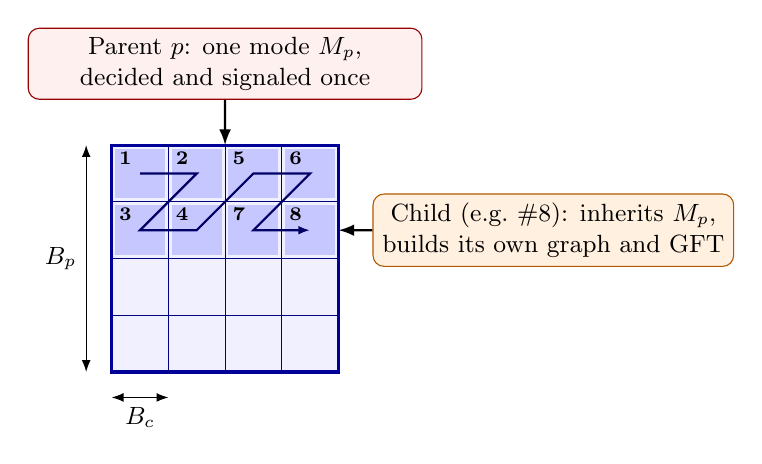
\begin{tikzpicture}[scale=0.72, every node/.style={font=\small}]
    \draw[draw=blue!60!black, very thick, fill=blue!6] (0,0) rectangle (4,4);
    \foreach \i in {1,2,3} {\draw[blue!50!black, thin] (\i,0)--(\i,4); \draw[blue!50!black, thin] (0,\i)--(4,\i);}
    \foreach \x/\y in {0/3, 1/3, 0/2, 1/2, 2/3, 3/3, 2/2, 3/2}
        \fill[blue!22] (\x+0.06,\y+0.06) rectangle (\x+0.94,\y+0.94);
    \draw[blue!40!black, thick, -{Latex[length=1.5mm]}]
        (0.5,3.5)--(1.5,3.5)--(0.5,2.5)--(1.5,2.5)--(2.5,3.5)--(3.5,3.5)--(2.5,2.5)--(3.5,2.5);
    \foreach \x/\y/\n in {0/3/1, 1/3/2, 0/2/3, 1/2/4, 2/3/5, 3/3/6, 2/2/7, 3/2/8}
        \node[font=\scriptsize\bfseries, anchor=north west, inner sep=1.5pt] at (\x+0.05,\y+0.97) {\n};
    \draw[{Latex[length=1.5mm]}-{Latex[length=1.5mm]}] (-0.45,0)--(-0.45,4) node[midway,left]{$B_p$};
    \draw[{Latex[length=1.5mm]}-{Latex[length=1.5mm]}] (0,-0.45)--(1,-0.45) node[midway,below]{$B_c$};
    \node[decbox, minimum width=5.0cm, anchor=south] (mode) at (2,4.8)
        {Parent $p$: one mode $M_p$,\\decided and signaled once};
    \draw[arr] (mode.south) -- (2,4);
    \node[attr, minimum width=4.4cm, anchor=west] (child) at (4.6,2.5)
        {Child (e.g.\ \#8): inherits $M_p$,\\builds its own graph and GFT};
    \draw[arr] (child.west) -- (4,2.5);
\end{tikzpicture}
\caption{Two-level hierarchical partition (2D cross-section): a parent block of side $B_p$
contains $(B_p/B_c)^3$ children of side $B_c$ (ratio 4 shown: 16 children in this slice).
Children are traversed in Morton order (blue path/numbering); the mode $M_p$ is decided and
signaled once per parent and inherited by every child. Colors as in Fig.~\ref{fig:operational}.}
\label{fig:hierarchy}
\end{figure}


\begin{figure}[t]
\centering
\resizebox{\linewidth}{!}{%
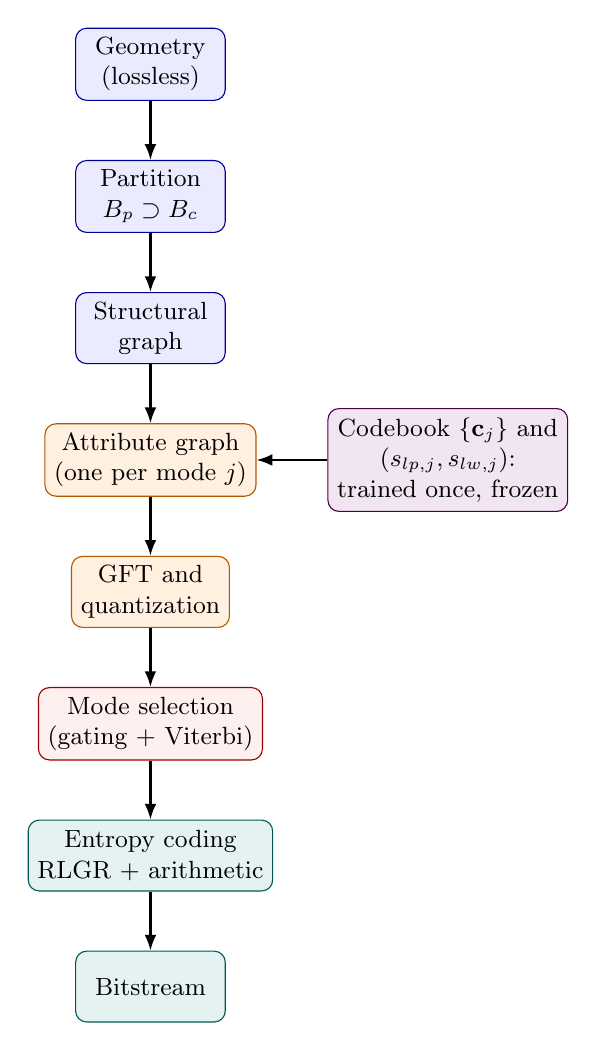
\begin{tikzpicture}[node distance=0.75cm and 0.4cm]
    \node[geo,  minimum width=1.9cm]                   (geom)  {Geometry\\(lossless)};
    \node[geo,  minimum width=1.9cm, below=of geom]    (part)  {Partition\\$B_p \supset B_c$};
    \node[geo,  minimum width=1.9cm, below=of part]    (struct){Structural\\graph};
    \node[attr, minimum width=2.3cm, below=of struct]  (attrg) {Attribute graph\\(one per mode $j$)};
    \node[attr, minimum width=1.9cm, below=of attrg]   (gft)   {GFT and\\quantization};
    \node[decbox, minimum width=2.3cm, below=of gft]   (sel)   {Mode selection\\(gating + Viterbi)};
    \node[bits, minimum width=2.3cm, below=of sel]     (ent)   {Entropy coding\\RLGR + arithmetic};
    \node[bits, minimum width=1.9cm, below=of ent]     (bs)    {Bitstream};
    \node[trained, minimum width=3.0cm, right=0.9cm of attrg] (cb)
          {Codebook $\{\mathbf c_j\}$ and\\$(s_{lp,j},s_{lw,j})$:\\trained once, frozen};
    \foreach \a/\b in {geom/part, part/struct, struct/attrg, attrg/gft, gft/sel, sel/ent, ent/bs}
        \draw[arr] (\a) -- (\b);
    \draw[arr] (cb) -- (attrg);
\end{tikzpicture}%
}
\caption{PCADC pipeline overview. Blue: geometry-only, lossless stages. Orange: stages that
depend on the attribute signal or its approximation. Violet: parameters trained once offline and
frozen. Red: per-block decision. Teal: entropy coding and bitstream. Same color code as
Figs.~\ref{fig:hierarchy}--\ref{fig:operational}.}
\label{fig:pipeline}
\end{figure}

\subsection{Directional Codebook and Self-Loop Graphs}
For each block, a tangent-plane linear fit of luminance against the block's two dominant
spatial axes (found by PCA) yields a 2D gradient $(s_1,s_2)$, which is embedded back into the
shared 3D frame as $\mathbf{g}_i = s_1\mathbf{q}_1 + s_2\mathbf{q}_2$. Its magnitude $g_i$
quantifies how pronounced the block's color gradient is; its unit direction
$\hat{\mathbf{g}}_i \in \mathbb{S}^2$ is the quantity clustered. Because only the axis of
variation matters (a gradient and its antipode describe the same surface orientation),
$K-1$ directional centroids $\{\mathbf{c}_j\}_{j=1}^{K-1}$ are trained by spherical $k$-means
under absolute cosine similarity $|\hat{\mathbf{g}}_i\cdot\mathbf{c}_j|$, restricted to the top
50\% of blocks by $g_i$ (near-planar blocks are excluded from training as unreliable). A
$K$-th, structural mode $j{=}0$ has no direction and no self-loops.

For a directional mode $j\ge1$, self-loops are added to a fraction $s_{lp}\in[0,1]$ of nodes
ranked by how strongly their local neighborhood decreases in the direction of $\mathbf{c}_j$
(reprojected onto that block's own tangent basis and scaled by its own $g_i$, so the mechanism
never requires the decoder to know the real color), each with weight $s_{lw}$:
\begin{equation}
    W_{ii} \leftarrow s_{lw}, \quad \forall i \in \mathcal{S}, \qquad
    |\mathcal{S}| = \lfloor s_{lp}\cdot N\rfloor .
\end{equation}
The resulting generalized Laplacian $L_g = D - A + C$ has a non-zero first eigenvalue and a
non-constant first eigenvector that down-weights self-looped nodes in the transform's DC term
-- the mechanism by which the graph, not just the quantizer, adapts to the signal.

\subsection{Offline Training and RDO Calibration}
Both the codebook directions and each mode's $(s_{lp,j}, s_{lw,j})$ are trained once per
sequence, on its first frame only, and frozen for all subsequent frames. This is deliberately
decoupled into two independent stages rather than a joint optimization: (1) directions are
found first, by spherical $k$-means; (2) for each direction already fixed, its self-loop
parameters are calibrated by a coarse $3\times3$ grid search over $(s_{lp},s_{lw})$, followed by
a golden-section refinement of $s_{lw}$ alone (a fixed, small number of iterations). An earlier
approach explored a joint 5-dimensional evolutionary optimization (direction and self-loops
together); it was abandoned in favor of this decoupled scheme because the latter is simpler,
orders of magnitude cheaper, and -- critically -- evaluable at the scale of the 14-sequence
benchmark reported below, which the joint approach never reached.

\subsection{Mode Selection: Gating and Viterbi}
\label{sec:mode-selection}
Figure~\ref{fig:operational} details how, at encode time, a parent block's mode $M_p$ is
decided once the codebook and self-loops are frozen. First, a gating barrier
$\tau_{\text{gate}}(Q)=\alpha_{\text{gate}}(Q/32)^2$ forces near-planar parent blocks
(luminance variance below $\tau_{\text{gate}}$) directly to the structural mode, without
evaluating any directional cost -- this keeps signaling cheap without being a cost-based
decision. Active blocks evaluate the full rate-distortion cost $J_j$ for every candidate mode
$j=0,\dots,K-1$ (graph, GFT, quantization for each child, aggregated over the parent), and a
Viterbi trellis then selects the mode sequence over the Morton-ordered sequence of active
parents, penalizing mode switches between neighboring blocks in proportion to how aligned their
normals are -- discouraging spurious switches with no underlying surface discontinuity. Child
blocks inherit their parent's mode and keep the coefficients already computed for it; the graph
is never rebuilt for the winning mode.

\begin{figure}[t]
\centering
\resizebox{\linewidth}{!}{%
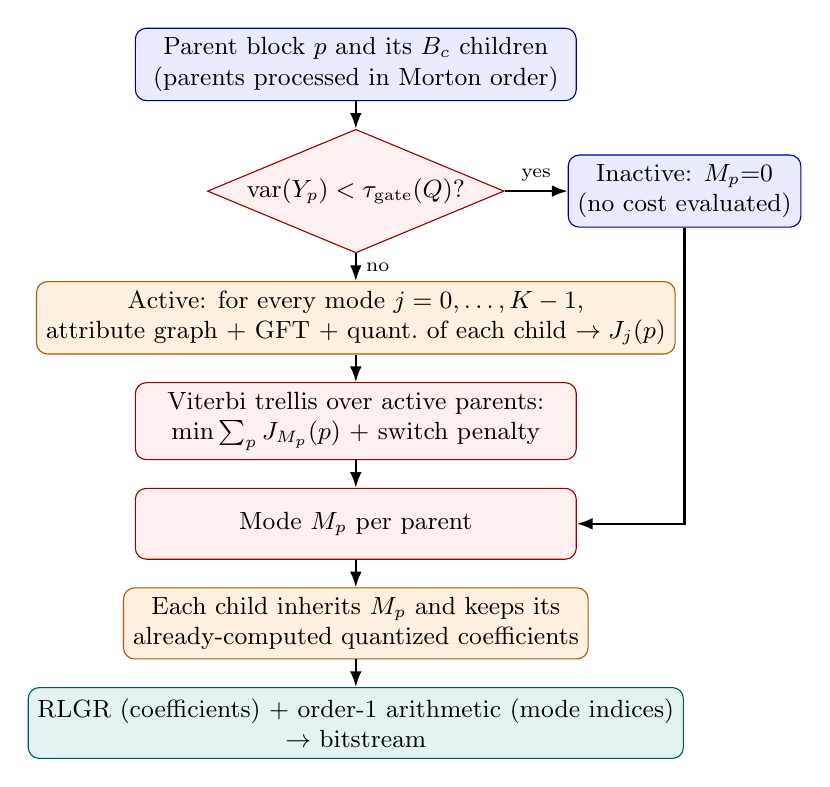
\begin{tikzpicture}[node distance=0.35cm and 0.8cm]
    \node[geo,  minimum width=5.6cm]                    (p)     {Parent block $p$ and its $B_c$ children\\(parents processed in Morton order)};
    \node[decision, below=of p]                         (gate)  {$\mathrm{var}(Y_p) < \tau_{\text{gate}}(Q)$?};
    \node[geo,  minimum width=2.6cm, right=0.8cm of gate] (inact) {Inactive: $M_p{=}0$\\(no cost evaluated)};
    \node[attr, minimum width=5.6cm, below=of gate]     (eval)  {Active: for every mode $j=0,\dots,K-1$,\\attribute graph + GFT + quant.\ of each child $\rightarrow J_j(p)$};
    \node[decbox, minimum width=5.6cm, below=of eval]   (vit)   {Viterbi trellis over active parents:\\$\min \sum_p J_{M_p}(p)$ + switch penalty};
    \node[decbox, minimum width=5.6cm, below=of vit]    (mp)    {Mode $M_p$ per parent};
    \node[attr, minimum width=5.6cm, below=of mp]       (inh)   {Each child inherits $M_p$ and keeps its\\already-computed quantized coefficients};
    \node[bits, minimum width=5.6cm, below=of inh]      (ent)   {RLGR (coefficients) + order-1 arithmetic (mode indices)\\$\rightarrow$ bitstream};
    \draw[arr] (p)--(gate);
    \draw[arr] (gate) -- node[right, font=\scriptsize] {no} (eval);
    \draw[arr] (gate) -- node[above, font=\scriptsize] {yes} (inact);
    \draw[arr] (eval)--(vit); \draw[arr] (vit)--(mp); \draw[arr] (mp)--(inh); \draw[arr] (inh)--(ent);
    \draw[arr] (inact.south) |- (mp.east);
\end{tikzpicture}}
\caption{Operational pipeline for each frame $t\geq1$, with codebook and self-loops already
frozen. Gating is applied before any cost is evaluated; for active parents the cost is computed
for \emph{every} candidate mode, and only then does the Viterbi trellis choose the mode
sequence -- the graph is never reconstructed for the winning mode. Colors as in
Fig.~\ref{fig:hierarchy}.}
\label{fig:operational}
\end{figure}

Only the mode index $M_p$ is signaled per parent block, coded with an order-1 adaptive
arithmetic coder conditioned on the immediately preceding parent's mode in Morton order --
exploiting real spatial redundancy in how modes are assigned, measured directly rather than
assumed (Sec.~\ref{sec:results}).

% =============================================================================
\section{Experimental Setup}
% =============================================================================
We evaluate on 14 real sequences from two standard dynamic point cloud datasets: 8iVFB
(\textit{longdress}, \textit{loot}, \textit{redandblack}, \textit{soldier}, octree depth 10) and
MVUB (five subjects, each captured at depth 9 and depth 10). Only the luminance ($Y$) channel is
GFT-coded and quantized; $U,V$ are lossless passthrough, following standard practice
(chroma subsampling in JPEG and most video codecs). The codebook and self-loops are trained on
frame 0 of each sequence and frozen for 5--7 additional evaluation frames sampled every 50
frames. The swept grid is $B_c\in\{4,8,16\}$ (with $B_p=32$ for depth-10 sequences and
$B_p=16$ for depth-9, so that $B_p$ always spans the same relative fraction of the bounding
box), $K\in\{4,8,16,24,30\}$, and $Q\in\{24,32,48,64\}$. The \textbf{baseline} in every
comparison is the same pipeline with the structural mode forced ($K{=}0$, no self-loops, no
adaptive selection): the exact ablation floor that isolates the contribution of signal-adaptive
self-loops from everything else in the pipeline. All reported numbers come from real RLGR and
order-1 arithmetic coding, including the signaling overhead; PSNR$_Y$ and BD-Rate/BD-PSNR
\cite{bjontegaard2001calculation} are computed on real coded bitstreams, never estimated.

% =============================================================================
\section{Results}
\label{sec:results}
% =============================================================================

\subsection{Rate-Distortion Curves}
Figure~\ref{fig:rd} shows RD curves for the same MVUB subject (\textit{phil}) at both available
octree depths, $B_c=16$, all trained codebook sizes $K$. Across all 42 (sequence, $B_c$) panels
evaluated in this study, the PCADC curve stays visibly above the purely structural baseline over
the entire tested $Q$ range, with no crossing at any operating point. The separation is largest
at small $Q$, where the method's ability to adapt non-flat frequency bases matters most, and
narrows as $Q$ grows and higher frequencies become irrelevant regardless of the basis used.

\begin{figure}[t]
\centering
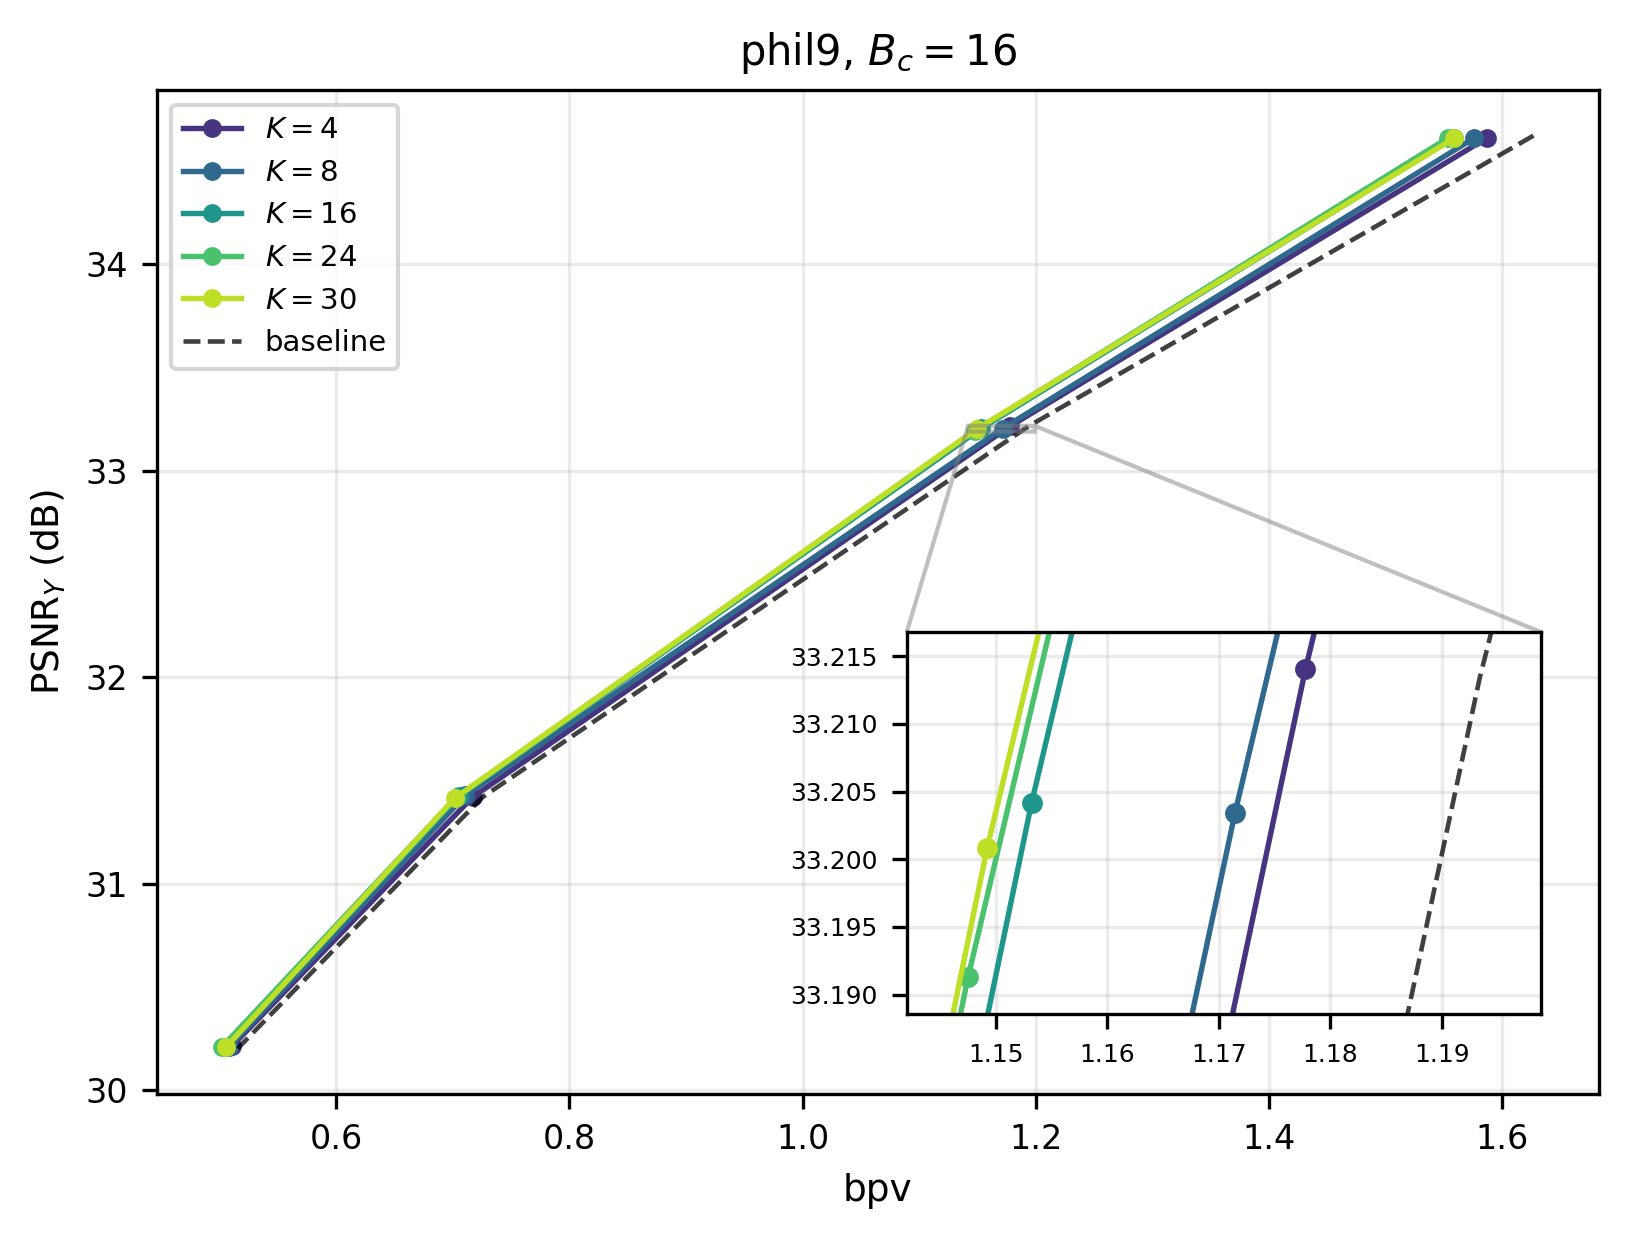
\includegraphics[width=0.49\linewidth]{e10_rd_phil9_bc16.png}\hfill
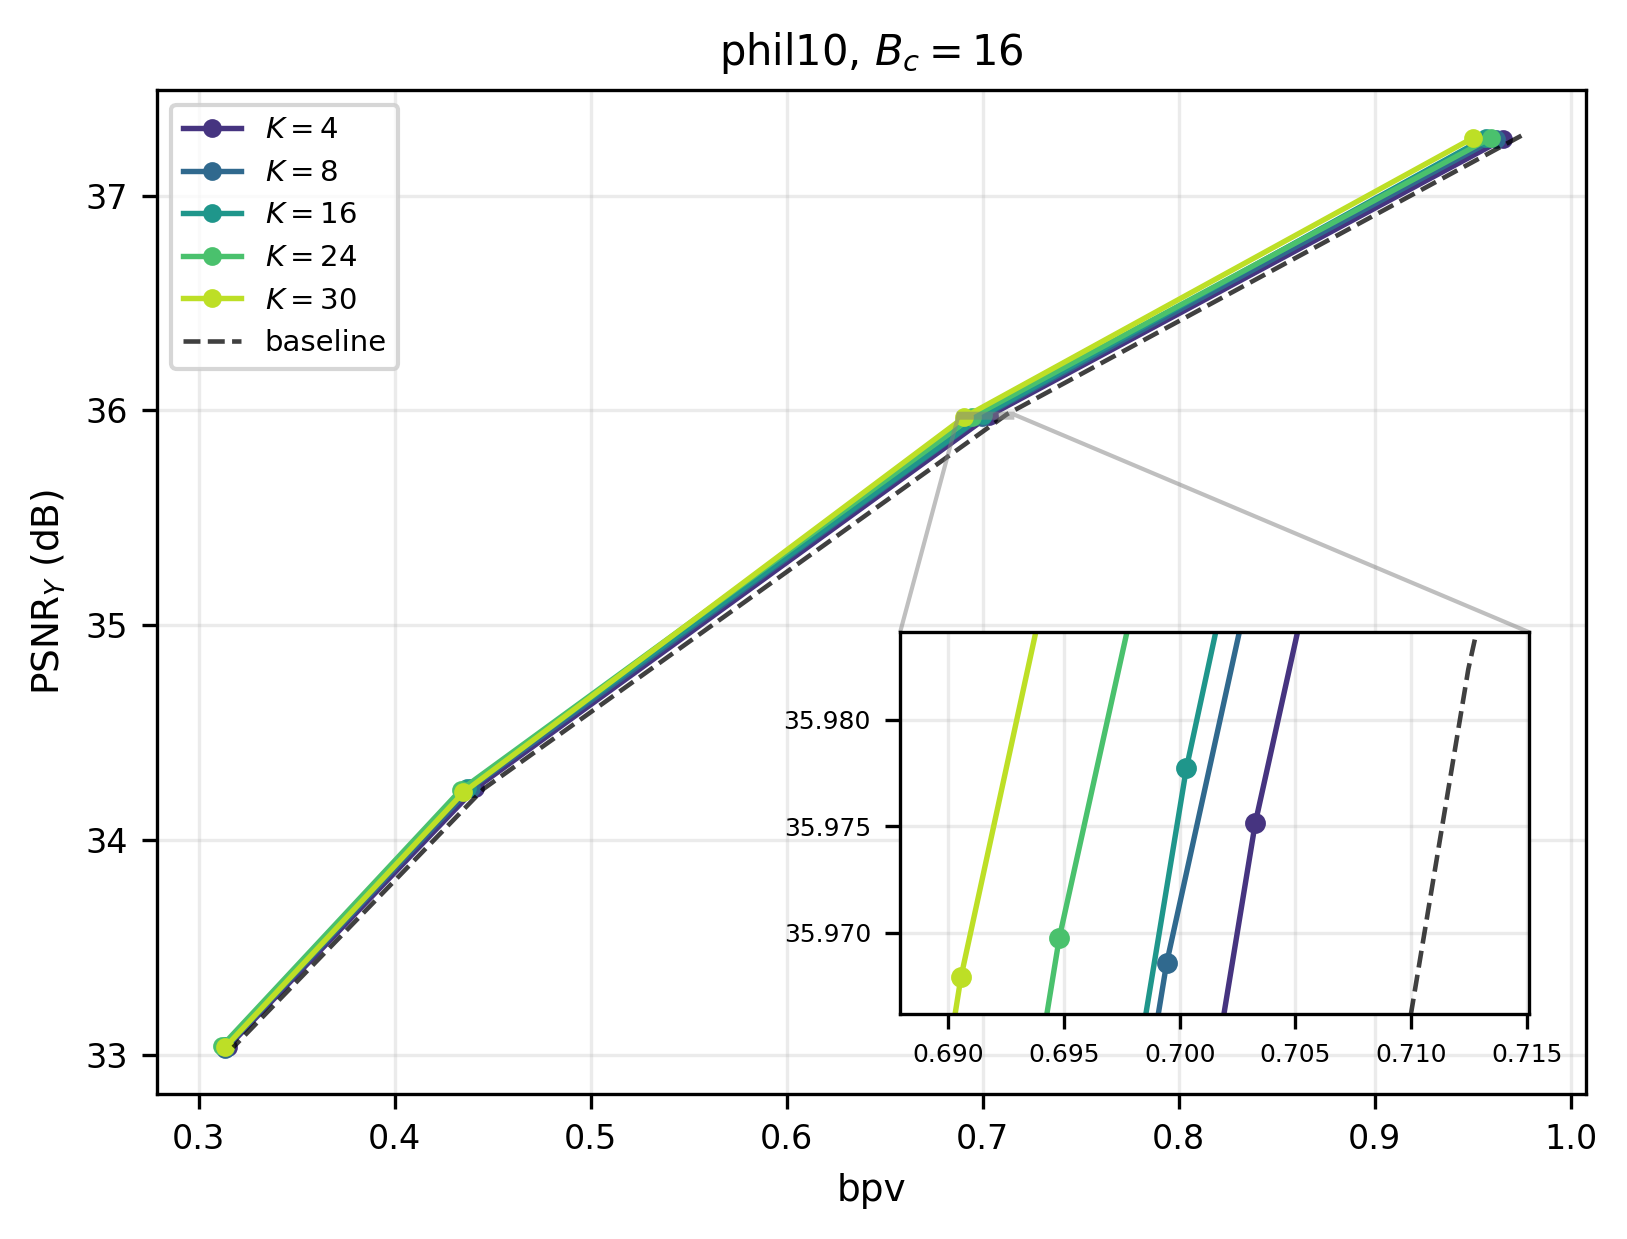
\includegraphics[width=0.49\linewidth]{e10_rd_phil10_bc16.png}
\caption{RD curves for the same subject (\textit{phil}) at $B_c=16$: depth 9 (left) vs.\ depth
10 (right), across trained codebook sizes $K$. The gap over the structural baseline (dashed
black) is wider at depth 9 -- the density/depth asymmetry discussed in
Sec.~\ref{sec:discussion}.}
\label{fig:rd}
\end{figure}

\subsection{BD-Rate Summary}
Table~\ref{tab:bdrate} reports BD-Rate/BD-PSNR for each sequence, at its best block size and
$K{=}24$, as mean$\pm$std over the evaluation frames. The average across all 14 sequences is
$-2.18\%$, with no sequence favoring the structural baseline. Depth-9 sequences gain
systematically more ($-2.98\%$ mean) than their depth-10 counterparts ($-1.74\%$ mean), and this
persists after controlling for the parent:child geometric ratio -- point density, not relative
resolution alone, drives the achievable gain.

\begin{table}[t]
\centering
\caption{BD-Rate / BD-PSNR at best $B_c$, $K{=}24$ (mean$\pm$std over evaluation frames).
Boldface: best overall result.}
\label{tab:bdrate}
\resizebox{\linewidth}{!}{%
\begin{tabular}{lccccc}
\toprule
Sequence & Family & Depth & $B_c$ & BD-Rate (\%) & BD-PSNR (dB) \\
\midrule
Longdress & 8iVFB & 10 & 16 & $-1.68 \pm 0.10$ & $+0.081 \pm 0.005$ \\
Loot & 8iVFB & 10 & 16 & $-1.56 \pm 0.11$ & $+0.061 \pm 0.004$ \\
Redandblack & 8iVFB & 10 & 16 & $-1.59 \pm 0.15$ & $+0.059 \pm 0.005$ \\
Soldier & 8iVFB & 10 & 16 & $-1.94 \pm 0.17$ & $+0.084 \pm 0.008$ \\
Andrew10 & MVUB & 10 & 8 & $-1.39 \pm 0.12$ & $+0.061 \pm 0.005$ \\
David10 & MVUB & 10 & 16 & $-1.54 \pm 0.35$ & $+0.061 \pm 0.016$ \\
Phil10 & MVUB & 10 & 16 & $-2.11 \pm 0.19$ & $+0.089 \pm 0.007$ \\
Ricardo10 & MVUB & 10 & 16 & $-1.45 \pm 0.16$ & $+0.069 \pm 0.007$ \\
Sarah10 & MVUB & 10 & 16 & $-2.38 \pm 0.26$ & $+0.102 \pm 0.012$ \\
Andrew9 & MVUB & 9 & 16 & $-2.76 \pm 0.36$ & $+0.138 \pm 0.018$ \\
David9 & MVUB & 9 & 16 & $-2.64 \pm 0.25$ & $+0.093 \pm 0.013$ \\
Phil9 & MVUB & 9 & 16 & $-3.28 \pm 0.17$ & $+0.149 \pm 0.008$ \\
Ricardo9 & MVUB & 9 & 16 & $-2.30 \pm 0.33$ & $+0.101 \pm 0.012$ \\
Sarah9 & MVUB & 9 & 16 & $\mathbf{-3.91 \pm 0.94}$ & $\mathbf{+0.172 \pm 0.043}$ \\
\midrule
\textbf{Average} & & & & $\mathbf{-2.18}$ & \\
\bottomrule
\end{tabular}}
\end{table}

\subsection{Signaling Overhead and Its Driver}
Overhead never exceeds $1.09\%$ of the bitstream across all 14
sequences and all evaluated configurations, and its dependence on $Q$ is explained directly by
the gating mechanism: the barrier $\tau_{\text{gate}}(Q)$ grows quadratically, forcing more
parent blocks to the zero-cost structural mode as quantization coarsens. More notably, overhead
is the single strongest correlate of BD-Rate across the 14 sequences ($r=-0.88$, $n{=}14$):
the sequences that spend the most on signaling are also the ones that gain the most, i.e., the
mode index is carrying information the coefficient coder actually exploits, not a fixed tax on
every sequence alike.

\subsection{Oracle Ceiling}
An exhaustive-search oracle, with perfect knowledge of the real luminance signal and no
signaling cost, bounds the mechanism's theoretical ceiling: $-17.31\%$ BD-Rate at block size
$B{=}4$, falling to $-6.75\%$ at $B{=}8$ and $-2.60\%$ at $B{=}16$. The real system captures
only a fraction of this ceiling, and -- notably -- in the opposite regime from where the oracle
is strongest: PCADC's real gain is largest at $B_c=16$ and smallest at $B_c=4$
($-0.18\%$ to $-0.61\%$), the reverse ordering of the oracle. Sec.~\ref{sec:discussion} explains
why.

% =============================================================================
\section{Discussion}
\label{sec:discussion}
% =============================================================================
The reversal between the oracle's and the real system's best block size is the central finding
of this work. The oracle can assign an unconstrained, per-child decision with zero signaling
cost, and is accordingly strongest exactly where the partition is finest. PCADC, by
construction, takes a single mode decision per \emph{parent} block and inherits it to every
child (Sec.~\ref{sec:mode-selection}) -- a design forced by the $O(N^2)$/$O(N^3)$ cost of
building a graph and its eigendecomposition at every candidate scale. As $B_c$ shrinks relative
to $B_p$, that one decision is inherited by children increasingly far, geometrically, from the
region it was actually optimized over, and the achievable gain collapses well before the
signaling budget (which stays under $1.1\%$ throughout) becomes the limiting factor. The method
does not fail at fine partitions; it pays for bounded signaling with decision resolution, and
that gap between the level at which the mode is decided and the level at which the transform is
applied is, at present, the method's principal limitation -- and the most direct target for
future work (e.g., an optional per-child refinement flag within the already-available signaling
budget).

A second, related observation is that the codebook is used near-uniformly by active blocks
rather than collapsing onto a few dominant directions, and that a first-order Markov model of
mode adjacency along the Morton order captures real, exploitable redundancy -- consistent with
the mode-continuity term in the Viterbi trellis being a genuine driver of the measured gain,
not merely a smoothing heuristic.

We report all of the above as a comparison against PCADC's own structural GFT baseline. No
external reference codec (e.g., RAHT under MPEG common test conditions) has been run against
the same 14 sequences; the bitstreams, PSNR protocol, and RD curves needed on the PCADC side
already exist, and closing this comparison is the most direct way to place the demonstrated
gain on an external scale.

% =============================================================================
\section{Conclusion}
% =============================================================================
We presented PCADC, a deterministic graph-transform scheme that adapts self-loops to the local
color gradient through an offline directional codebook, achieving a consistent $-2.18\%$ average
BD-Rate over a purely structural GFT baseline across 14 real sequences, with bounded
($\le1.09\%$) and informative signaling overhead. An oracle analysis shows the mechanism's
theoretical ceiling reaches $-17.31\%$ at fine block sizes, and identifies the distance between
the scale at which the mode is decided and the scale at which the transform is applied as the
main reason the real system captures only part of that ceiling -- and where its largest
remaining gain is likely to come from. The contribution here is not the magnitude of the
reported gain, which is modest against that ceiling, but a real, measured, and interpretable
mechanism for turning attribute-signal structure into compression gain, together with a precise
account of where the rest of that gain is currently lost.

% =============================================================================
\begin{thebibliography}{00}

\bibitem{zhang2014point}
C. Zhang, D. Florêncio, and C. Loop, ``Point cloud attribute compression with graph transform,''
in \emph{Proc. IEEE Int. Conf. Image Process. (ICIP)}, 2014, pp. 2066--2070.

\bibitem{pavez2020region}
E. Pavez, B. Kathariya, A. Ortega, and J. Chou, ``Region adaptive graph Fourier transform for
3D point clouds,'' \emph{IEEE Trans. Signal Process.}, 2020.

\bibitem{dequeiroz2016raht}
R. L. de Queiroz and P. A. Chou, ``Compression of 3D point clouds using a region-adaptive
hierarchical transform,'' \emph{IEEE Trans. Image Process.}, vol. 25, no. 8, pp. 3947--3956,
2016.

\bibitem{graziosi2020overview}
D. Graziosi, O. Nakagami, S. Kuma, A. Zaghetto, T. Suzuki, and A. Tabatabai, ``An overview of
ongoing point cloud compression standardization activities: video-based (V-PCC) and
geometry-based (G-PCC),'' \emph{APSIPA Trans. Signal Inf. Process.}, vol. 9, e13, 2020.

\bibitem{egilmez2017graphlearning}
H. E. Egilmez, E. Pavez, and A. Ortega, ``Graph learning from data under Laplacian and
structural constraints,'' \emph{IEEE J. Sel. Topics Signal Process.}, vol. 11, no. 6, pp.
825--841, 2017.

\bibitem{quach2019learning}
M. Quach, G. Valenzise, and F. Dufaux, ``Learning convolutional transforms for lossy point
cloud geometry compression,'' in \emph{Proc. IEEE Int. Conf. Image Process. (ICIP)}, Taipei,
2019, pp. 4320--4324.

\bibitem{sheng2021deeppcac}
X. Sheng, L. Li, D. Liu, Z. Xiong, Z. Li, and F. Wu, ``Deep-PCAC: An end-to-end deep lossy
compression framework for point cloud attributes,'' \emph{IEEE Trans. Multimedia}, vol. 24, pp.
2617--2632, 2022.

\bibitem{fang2022_3dac}
G. Fang, Q. Hu, H. Wang, Y. Xu, and Y. Guo, ``3DAC: Learning attribute compression for point
clouds,'' in \emph{Proc. IEEE/CVF Conf. Comput. Vis. Pattern Recognit. (CVPR)}, 2022, pp.
14819--14828.

\bibitem{bjontegaard2001calculation}
G. Bj\o ntegaard, ``Calculation of average PSNR differences between RD-curves,'' ITU-T
SG16/Q6 VCEG, Doc. VCEG-M33, Austin, TX, 2001.

\bibitem{dhillon2001concept}
I. S. Dhillon and D. S. Modha, ``Concept decompositions for large sparse text data using
clustering,'' \emph{Mach. Learn.}, vol. 42, no. 1, pp. 143--175, 2001.

\bibitem{viterbi1967error}
A. J. Viterbi, ``Error bounds for convolutional codes and an asymptotically optimum decoding
algorithm,'' \emph{IEEE Trans. Inf. Theory}, vol. 13, no. 2, pp. 260--269, 1967.

\bibitem{marpe2003cabac}
D. Marpe, H. Schwarz, and T. Wiegand, ``Context-based adaptive binary arithmetic coding in the
H.264/AVC video compression standard,'' \emph{IEEE Trans. Circuits Syst. Video Technol.}, vol.
13, no. 7, pp. 620--636, 2003.

\bibitem{ortega1998rate}
A. Ortega and K. Ramchandran, ``Rate-distortion methods for image and video compression,''
\emph{IEEE Signal Process. Mag.}, vol. 15, no. 6, pp. 23--50, 1998.

\bibitem{ortega2022gsp}
A. Ortega, \emph{Introduction to Graph Signal Processing}. Cambridge Univ. Press, 2022.

\bibitem{loop2016microsoft}
C. Loop, Q. Cai, S. Choisnard, and P. A. Chou, ``Microsoft voxelized upper bodies -- a point
cloud dataset,'' ISO/IEC JTC1/SC29/WG11 (MPEG), Doc. m38673, 2016.

\end{thebibliography}

\end{document}
